%!TEX root = ../var.tex
\begin{definition}
\label{def:12.1}
	Случайная величина $\xi$ называется абсолютно непрерывной, если существует такая неотрицательная функция $f_{\xi} (x)$ (возможно обобщённая, см. §13), что для любого $x \in \mathbb{R}$ функция распределения $F_{\xi}(x)$ представима в виде\footnote{В дальнейшем мы рассматриваем только такие случайные величины, для которых все связанные с
ними несобственные интегралы и суммы бесконечных рядов сходятся абсолютно.
	}
  
\begin{equation*}
	F_{\xi}(x)=\int_{-\infty}^{x} f_{\xi}(t) dt  	
\end{equation*}

При этом функция $f_{\xi}(x)$ называется плотностью вероятности случайной величины $\xi$
\end{definition}

\begin{zam}
\label{zam:12.2}
Если $F_{\xi}(x)$ -- дифференцируемая функция распределения, то название "плотность вероятности" имеет следующее объяснение. С одной стороны, используя формулу дифференцирования интеграла по верхнему пределу, имеем $\frac{dF_{\xi}(x)}{dx}=f_{\xi}(t)|_t=x$. С другой стороны, по определению производной имеем:

\begin{gather*}
	\frac{dF_{\xi}(x)}{dx} = \frac{F_{\xi}(x+dx)-F_{\xi}(x)}{dx}=\frac{\P(\xi \leq x+dx)-\P(\xi \leq x)}{dx}=\\=\frac{\P(\{\xi \leq x+dx \}\ssm \{\xi \leq x\})}{dx} = \frac{\P(x<\xi \leq x+dx)}{dx}
\end{gather*}
Поэтому

\begin{equation*}
	f_{\xi}(x)=\frac{\P(x,\xi \leq x+dx)}{dx}	
\end{equation*}
есть отношение вероятности попадания случайной величины $\xi$ в интервал $(x, x+dx]$ к длине этого интервала $dx$, что физически означает плотность вероятности (<<массы>>) случайной величины $\xi$ в точке $x$.
\end{zam}
 

 \begin{theorem}
 \label{th:12.3}
Плотность обладает свойствами:

1) $f_{\xi}(x) \geq 0$ для любого $x$;

2) $\int\limits_{-\infty}^{\infty} f_{\xi}(t)dt=1$
 \end{theorem}

\begin{proof}

1) По теор. 11.4.1 функция распределения $F_{\xi}(x)$ -- неубывающая, поэтому $\frac{dF_{\xi}(x)}{dx}=f_{\xi}(x) \geq 0$

2) $\int\limits_{-\infty}^{\infty}f_{\xi}(t)dt = lim_{x \to \infty}\int\limits_{-\infty}^{x}f_{\xi}(t)dt = \lim\limits_{x \to \infty}F_{\xi}(x) = 1$ по свойству 11.4.2.
\end{proof} 

\begin{definition}
 \label{def:12.4}

Пусть область $U \subseteq \mathbb{R}^n$ имеет меру $\mu(U )$. Говорят, что в области $U$ функция $h : U \to \mathbb{R}$ удовлетворяет некоторому свойству $\mathcal{P}$ почти всюду, если подмножество $A \subset U$ , в котором свойство $\mathcal{P}$ не выполняется, имеет меру 0, т.е. $\mu(A) = 0$.
Докажем свойства абсолютно непрерывных случайных величин.
\end{definition}

\begin{theorem}
 \label{th:12.5}

Если случайная величина $\xi$ абсолютно непрерывна, то

1) её функция распределения $F_{\xi}(x)$ непрерывна в $\mathbb{R}$ и дифференцируема почти всюду в $\mathbb{R}$, т.е. равенство $f_{\xi}(x) = \frac{d}{dx}F_{\xi}(x)$ справедливо почти всюду,

2) $\P(\xi = x) = 0$ для любого $x \to \mathbb{R}$,

3) $\P(a \leq \xi < b) = \P(a < \xi < b) = \P(a \leq \xi \leq b) = \P(a < \xi \leq b) = \int_{a}^{b}f_{\xi}(t)dt.$
\end{theorem}

\begin{proof}
1) Во-первых, функция $F_{\xi}(x) = \int_{-\infty}^{x}f_{\xi}(t)dt$ непрерывна как функция верхнего предела интеграла.
Во-вторых, по теор. \ref{th:11.5} функция $F_{\xi}(x)$ имеет не более чем счётное множество скачков, поэтому она не дифференцируема не более чем в счётном
множестве точек. Любое счётное множество точек на прямой имеет нулевую меру (длину). Поэтому $F_{\xi}(x)$ дифференцируема почти всюду в $\mathbb{R}$.

2) Это следует из \ref{th:11.6}.3).

3) Из \ref{th:11.6}.4) имеем
$$\P(a < \xi \leq b) = F_{\xi}(b) - F_{\xi}(a) = \int_{-\infty}^{b}f_{\xi}(t)dt - \int_{-\infty}^{a}f_{\xi}(t)dt = \int_{a}^{b}f_{\xi}(t)dt$$

\end{proof}
Остальные равенства следуют из \ref{consq:11.7}.

\vspace{1em}\textbf{Примеры абсолютно непрерывных случайных величин}

\begin{definition}
 \label{def:12.6}

Случайная величина $\xi$ имеет равномерное распределение на отрезке $a, b$, если

\begin{equation*}
	F_{\xi}(x) = \P(\xi \leq x) = 
	\left\{
	\begin{aligned}
		0, & x<a\\
		\frac{x-a}{b-a}, & a \leq x \leq b\\
		1, & x>b\\
	\end{aligned}\right. \text{ и } f_{\xi}(x) = 
	\left\{
	\begin{aligned}
		0, & x<a\\
		\frac{1}{b-a}, & a \leq x \leq b\\
		1, & x>b\\
	\end{aligned}\right.
\end{equation*}

Графики функций $F_{\xi}(x)$ и $f_{\xi}(x)$ показаны на рис. 13. Заметим, что в точках $a$ и $b$ функция распределения $F_{\xi}(x)$ не дифференцируема, поэтому значение плотности вероятности в этих точках можно задать как угодно: либо $f_{\xi}(a) = 0$, либо $f_{\xi}(a) = \frac{1}{b-a}$, а на другом конце тоже либо $f_{\xi}(b) = 0$, либо $f_{\xi}(b) = \frac{1}{b-a}$
\end{definition}
	
\begin{definition}
 \label{def:12.7}
Случайная величина $\xi$ имеет показательное распределение с параметром $\lambda$ (рис. 14), если

\begin{equation*}
	f_{\xi}(x) = 
	\left\{
	\begin{aligned}
		0, & x<0\\
		\lambda e^{-\lambda x}, & x \geq 0\\
	\end{aligned}\right.
\end{equation*}
\end{definition}

\begin{figure}[H]
	\centering
	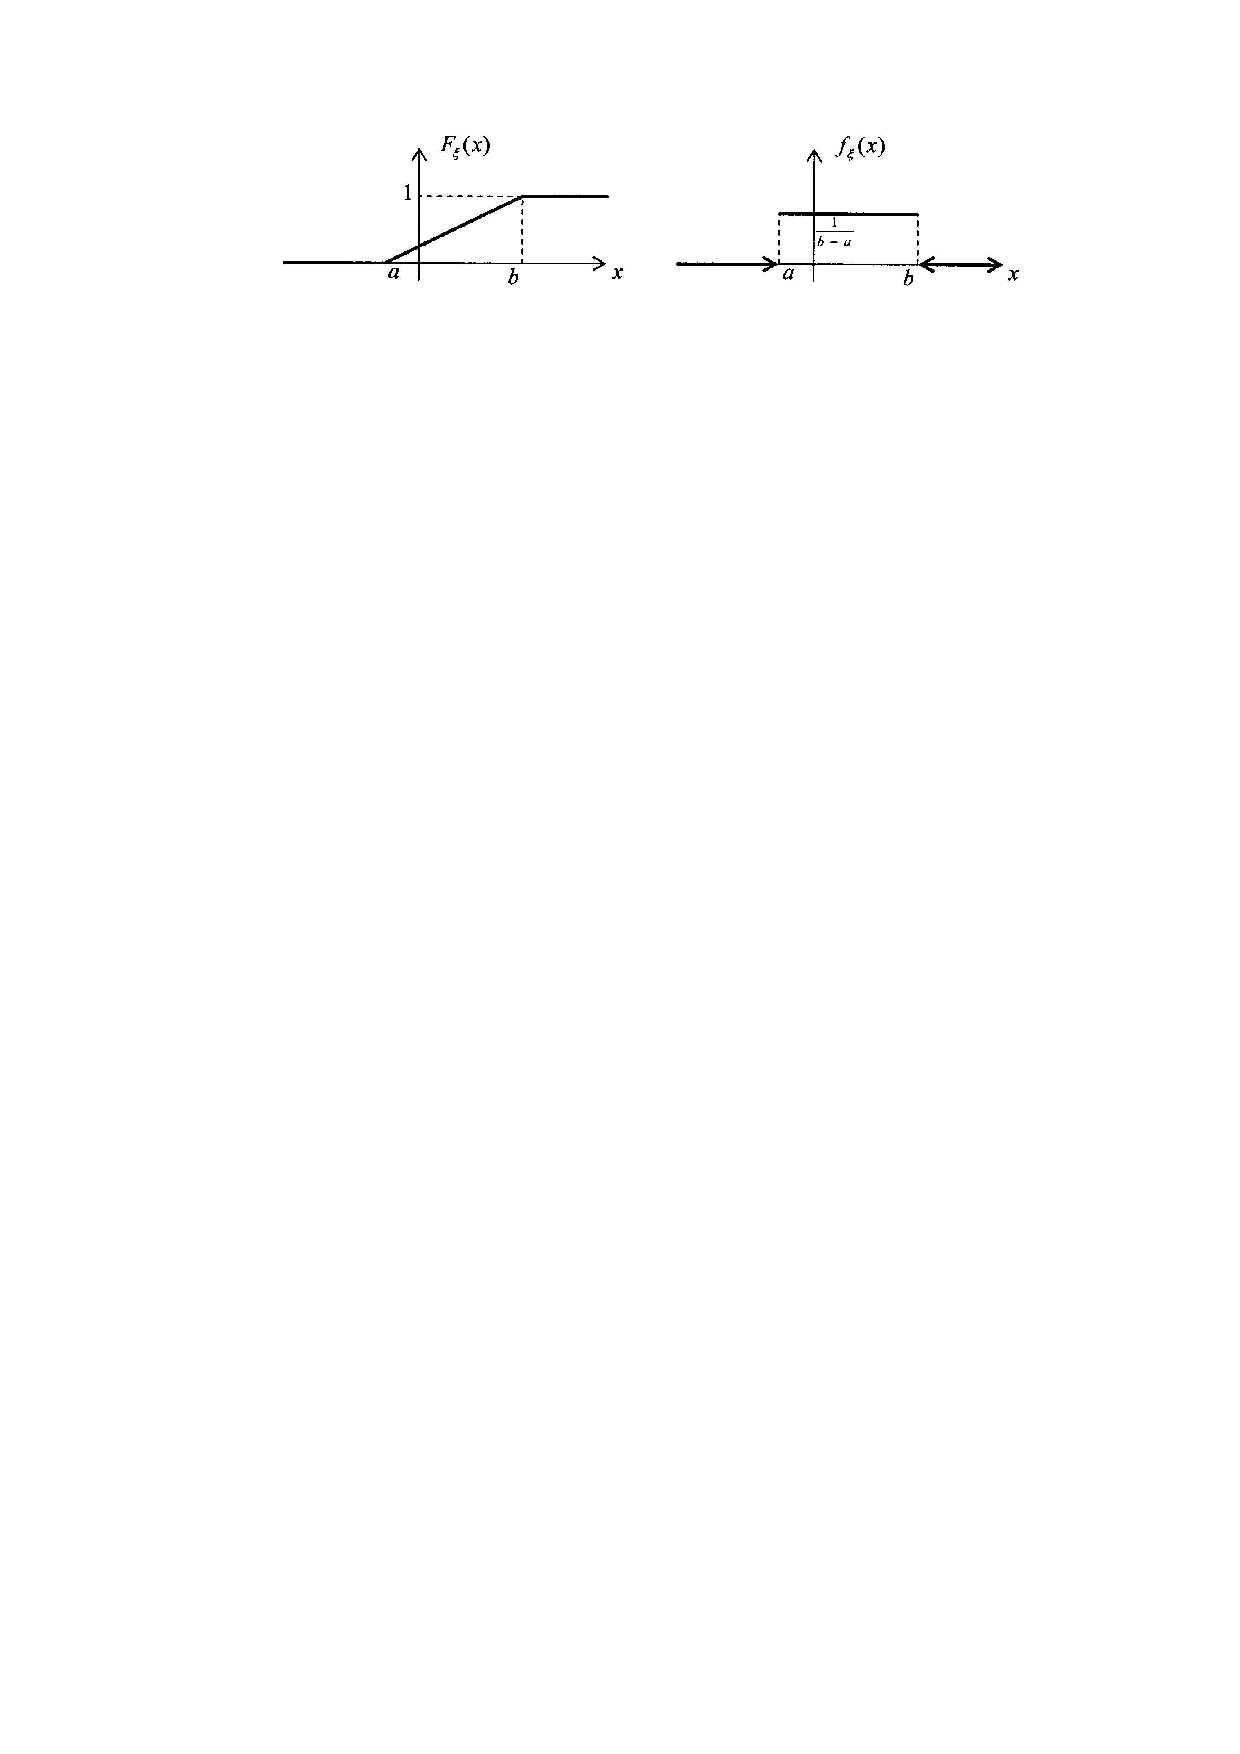
\includegraphics[]{pic/pic13}
	\caption{Равномерное распределение}
	\label{fig13}
\end{figure}
\begin{figure}[H]
	\centering
	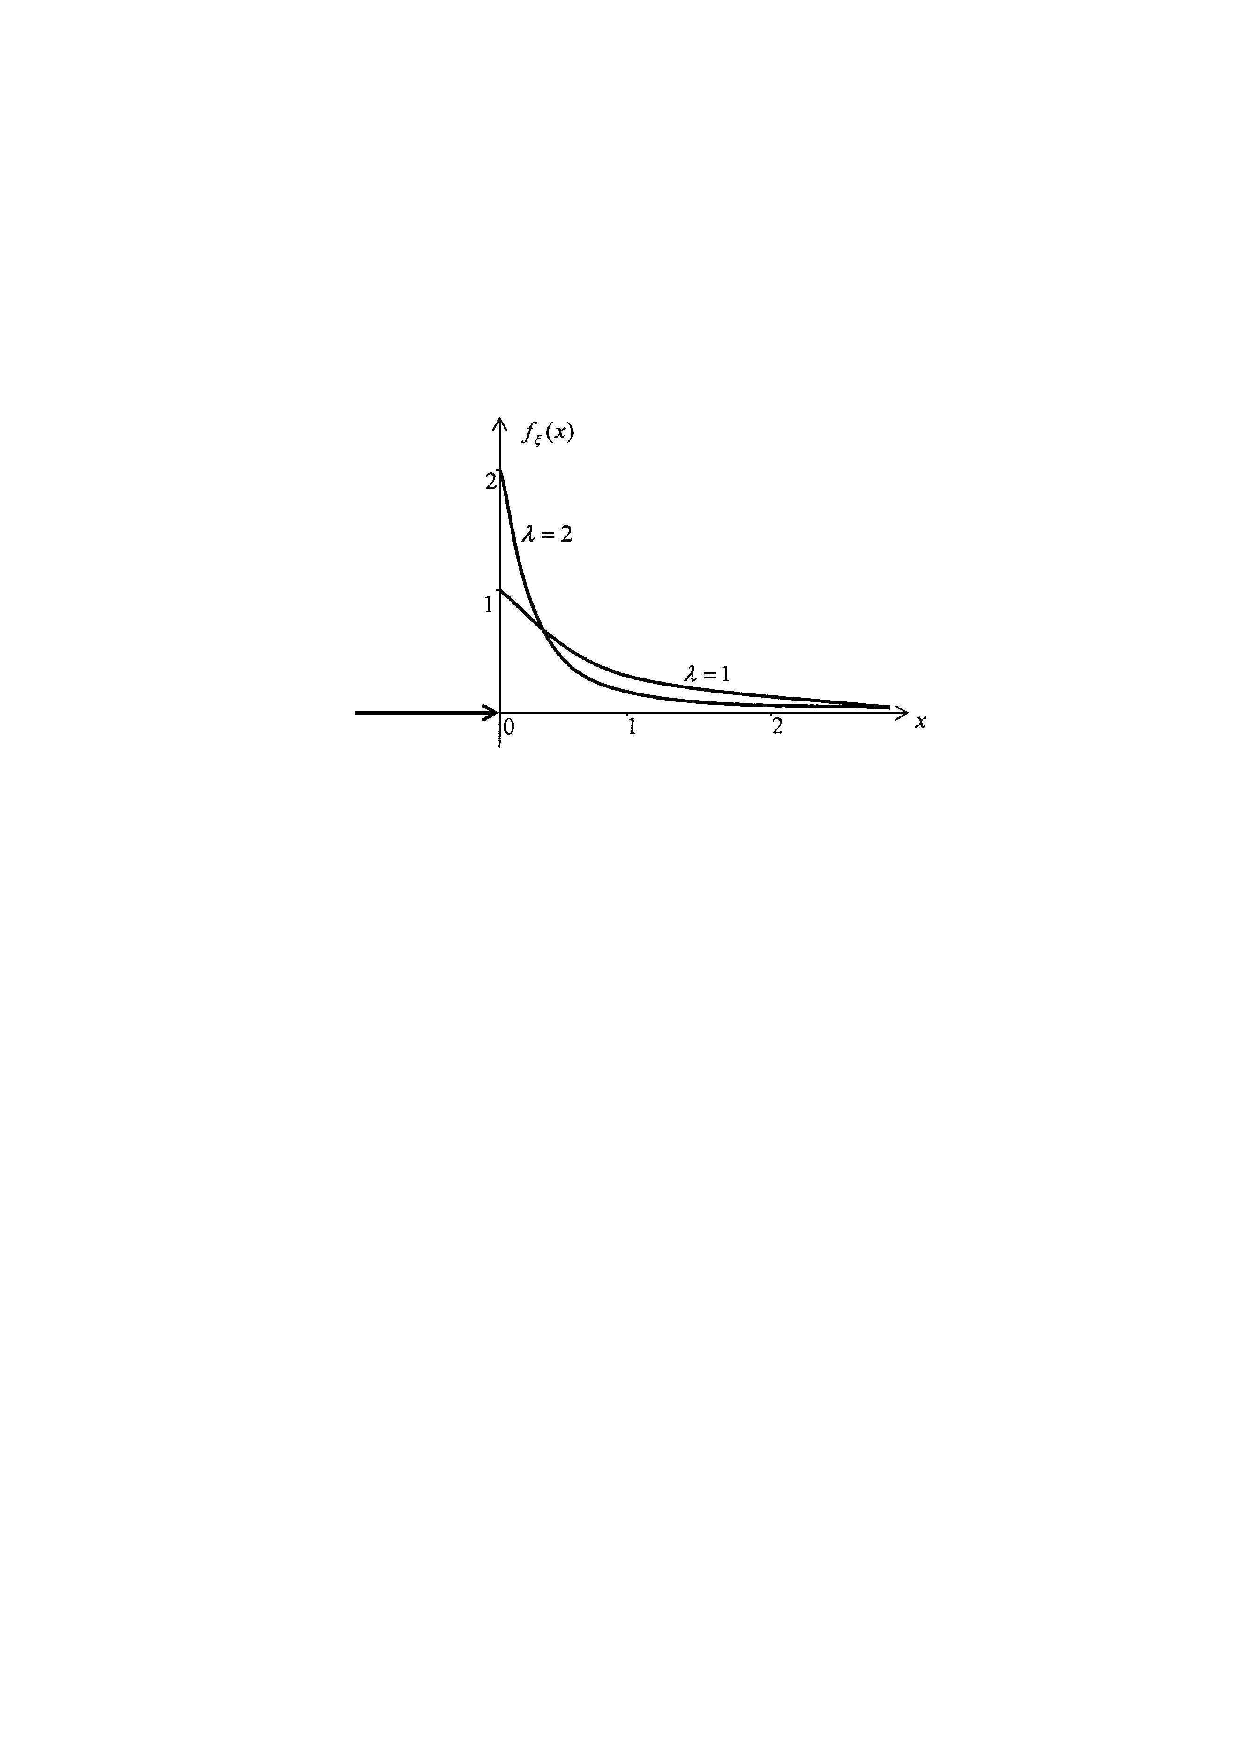
\includegraphics[]{pic/pic14}
	\caption{Показательное распределение}
	\label{fig14}
\end{figure}

\begin{definition}
 \label{def:12.8}
Если для любого $x \in \mathbb{R}$ случайная величина $\xi$ имеет плотность
\begin{equation*}
	f_{\xi}(x) = \frac{1}{2 \sqrt{2\pi}}e^{-\frac{(x-a)^2}{2\sigma^2}},
\end{equation*}

то говорят, что $\xi$ имеет нормальное (или Гаусса\footnote{
Карл Фридрих Гаусс (Johann Carl Friedrich Gauß, 1777 — 1855), выдающийся немецкий математик,
астроном и физик, считается одним из величайших математиков всех времён.	
} 
) распределение с математическим ожиданием $a$ и дисперсией $\sigma^2$ , где $a \in \mathbb{R}$ и $\sigma > 0$. (См. рис. 15) Очевидно, что $f_{\xi}(x) \geq 0$ для любого $x$;

2) Используем табличный интеграл (Пуассона)
$\int_{-\infty}^{\infty}e^{-\frac{t^2}{2}}dt=\sqrt{2\pi}$.

\begin{gather*}
	\int_{-\infty}^{\infty} f_{\xi}(x)dx = \int_{-\infty}^{\infty} \frac{1}{\sigma \sqrt{2\pi}}e^{-\frac{(x-a)^2}{2\sigma^2}}dx =
	%
	\left[
	\begin{aligned}
		\text{замена переменных}\\
		t = \frac{x-a}{\sigma}, dx = \sigma dt
	\end{aligned}\right]=\\=
	\frac{1}{\sqrt{2\pi}}\int_{-\infty}^{\infty}e^{-\frac{t^2}{2}}dt=1.
\end{gather*}
\end{definition}

\begin{prop}
 \label{prop:12.9}
 Легко сосчитать, что расстояние между точками перегиба равно $2\sigma$, поэтому параметр $2\sigma$ является характеристикой ширины графика на уровне точек перегиба.

\begin{figure}[H]
	\centering
	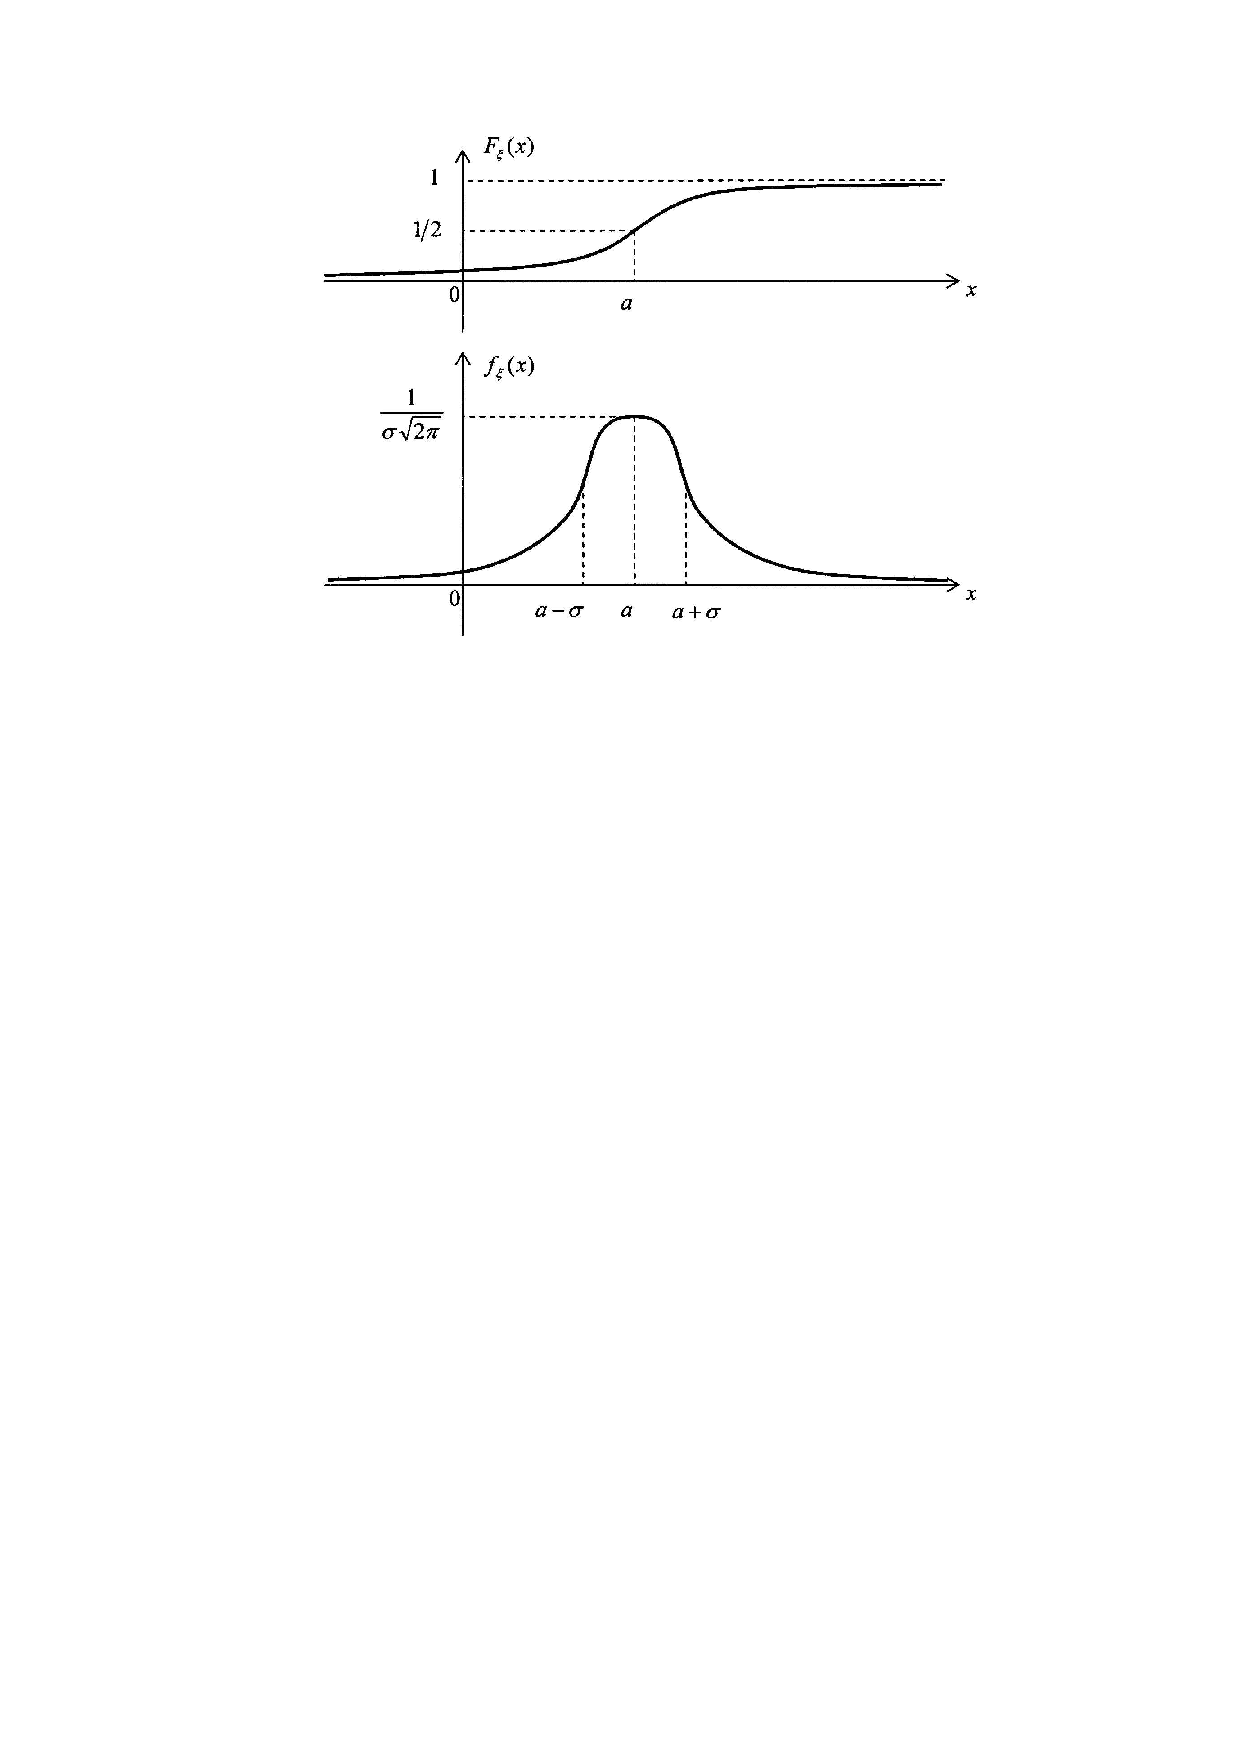
\includegraphics[]{pic/pic15}
	\caption{Нормальное распределение (Гаусса)}
	\label{fig15}
\end{figure}
 Заметим, что вероятность попадания  нормальной случайной величины в интервал между точками перегиба
\begin{equation*}
	\P(a − \sigma \leq \xi \leq a + \sigma) = \frac{1}{\sigma \sqrt{2\pi}} \int_{a-\sigma}^{a+\sigma} e^{-\frac{(x-a)^2}{2\sigma^2}}dx =  \frac{1}{\sigma \sqrt{2\pi}} \int_{-1}^{1} e^{-\frac{t^2}{2}}dt = 2\Phi(1) \approx 0.6827
\end{equation*}

где $\Phi(1)$ приближённое значение функции $\Phi (x) = \frac{1}{\sqrt{2\pi}} \int_{0}^{x}e^{-\frac{t^2}{2}}dt$
взято из таблицы.
\end{prop}

\begin{prop}[<<Правило трёх сигм>>]
 \label{prop:12.10}
Если $\xi$ — нормальная случайная величина, то $\P(|\xi − a| \leq 3\sigma) = 2\Phi(3) \approx 2\cdot0.49865 \approx 0,997$. Запоминать число $0,997$ нет никакого смысла, а вот помнить, что почти вся вероятность (<<масса>>) нормального распределения сосредоточена в интервале $[a − 3\sigma, a + 3\sigma]$, всегда полезно.
\end{prop}
